\begin{frame}
	\frametitle{Desarrollo de la Aplicación}
	\block{Clases Principales}
		\begin{itemize}
			\item Clase {\ttfamily Student}.
			\item Clase {\ttfamily Father}.
			\item Clase {\ttfamily Teacher}.
			\item Clase {\ttfamily Message}.
		\end{itemize}
	\endblock{}
\end{frame}

%--------------------------------------------------------------------

%¿Quitar?
\begin{frame}
	\frametitle{Ejemplo {\ttfamily Student}}
	\lstinputlisting{Code/Student.java}
\end{frame}

%--------------------------------------------------------------------

\begin{frame}
	\frametitle{Ejemplo {\ttfamily Student}}
	\lstinputlisting{Code/StudentParcelable.java}
\end{frame}

%--------------------------------------------------------------------

\begin{frame}
	\frametitle{Base de datos en el dispositivo {\ttfamily MessageSQLHelper}}
	\block{Tabla Conversations}
		\begin{itemize}
			\item Id (Clave primaria).
			\item D.N.I del destinatario.
			\item D.N.I del remitente.
		\end{itemize}
	\endblock{}
	\block{Tabla Messages}
		\begin{itemize}
			\item Id (Clave Primaria).
			\item Id de la conversación.
			\item D.N.I del remitente.
			\item Nombre del remitente.
			\item Datos del del envío del mensaje.
		\end{itemize}
	\endblock{}
\end{frame}

%--------------------------------------------------------------------

\begin{frame}
	\frametitle{Ejemplo {\ttfamily MessageSQLHelper}}
	\lstinputlisting{Code/MessageSQLHelper.java}
\end{frame}

%--------------------------------------------------------------------

\begin{frame}
	\frametitle{Interacción con la base de datos en {\it Firebase}}
	\block{Base de datos en la nube}
		\begin{enumerate}
			\item En {\ttfamily app/build.gradle} añadir:
				\begin{itemize}
					\item {\ttfamily compile 'com.firebase:firebase-client-android 2.2.1'}
				\end{itemize}
			\item Importar los servicios a usar en los archivos de clase ({\ttfamily java}).
			\item  En {\ttfamily onCreate()} incorporar:
				\begin{itemize}
					\item {\ttfamily Firebase.setAndroidContext(this)}
				\end{itemize}
			\item Colocar una referencia a la base de datos o a una de sus tablas.
			\item Crear la consulta.
			\item situar un {\it oyente} ({\ttfamily listener}).
		\end{enumerate}
	\endblock{}
\end{frame}

%--------------------------------------------------------------------

\begin{frame}
	\frametitle{Ejemplo interacción con la base de datos (Obtener datos)}
	\lstinputlisting{Code/StudentActivity.java}
\end{frame}

%--------------------------------------------------------------------

\begin{frame}
	\frametitle{Ejemplo interacción con la base de datos (Almacenar datos)}
	\lstinputlisting{Code/AddChildActivity.java}
\end{frame}

%--------------------------------------------------------------------

\begin{frame}
	\frametitle{Idiomas}
	\begin{center}
		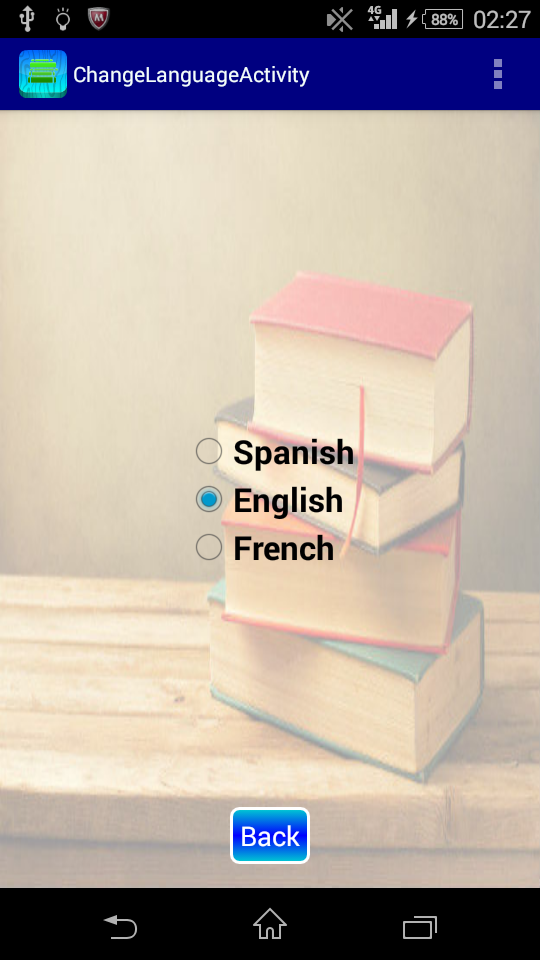
\includegraphics[width=0.3\linewidth]{Images/App/ChangeLanguaje}
	\end{center}
\end{frame}

%--------------------------------------------------------------------

\begin{frame}
	\frametitle{Idiomas}
	\lstinputlisting{Code/ChangeLanguageActivity.java}
\end{frame}

%--------------------------------------------------------------------

\begin{frame}
	\begin{center}
		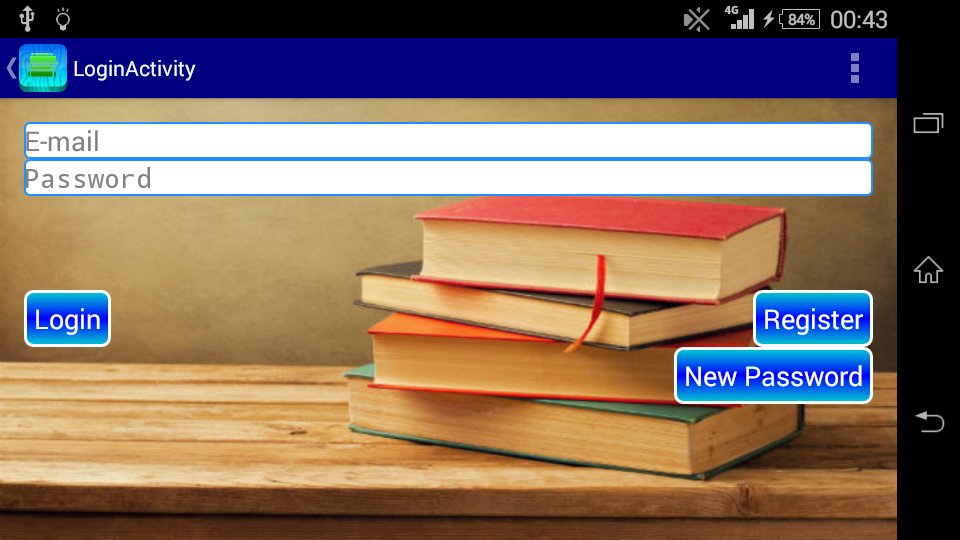
\includegraphics[width=0.7\linewidth]{Images/App/loginLand}
	\end{center}
\end{frame}